\documentclass[a4paper,pdf]{article} 
\usepackage{hyperref}
\usepackage{pdfpages}
\usepackage{booktabs} 
\usepackage{lineno}
\linenumbers  

\usepackage[utf8]{inputenc}
\usepackage[english]{babel}
\usepackage{amsmath}
\usepackage{graphicx}
\usepackage[colorinlistoftodos]{todonotes} % handig voor commentaar: gebruik \todo{}, zie ftp://ftp.fu-berlin.de/tex/CTAN/macros/latex/contrib/todonotes/todonotes.pdf
\usepackage{listings}
\usepackage{pdfpages}
\usepackage{tcolorbox}
\usepackage{float}
\usepackage{caption}
\usepackage{subcaption}
\usepackage{array}
\usepackage{pgfgantt}
\usepackage{graphicx}
\graphicspath{ {./images/} }
\usepackage[square,numbers]{natbib}
\bibliographystyle{abbrvnat}

\title{Bibliography management: \texttt{natbib} package}
\author{Share\LaTeX}
\date { }

\begin{document}

\title{“When the looting starts, the shooting starts": An analysis of hate speech on Twitter\\
\large  According to multi-label text classification with Swivl and BERT} 
\author{Kimberley van Ruiven}

\maketitle

\todototoc
\listoftodos
\tableofcontents

\begin{abstract}XXX
\todo{rewrite abstract}

\end{abstract}

\section{Personal details}

\begin{description}
 \item[My email:] \url{ kimberley.vanruiven@uva.nl }
 \item[My supervisors email:] \url{r.gopalakrishnapillai@uva.nl }
 \item[The wiki on my github account:] \url{https://github.com/pastatimes/Master-Thesis-Trump-tweets}
 \end{description} 

\section{Introduction}


    '....These THUGS are dishonoring the memory of George Floyd, and I won’t let that happen. Just spoke to Governor Tim Walz and told him that the Military is with him all the way. Any difficulty and we will assume control but, when the looting starts, the shooting starts. Thank you!'
    — Donald J. Trump (@realDonaldTrump) May 29, 2020 \footnote{https://twitter.com/realDonaldTrump/status/1266231100780744704?ref_src=twsrc} \\ \todo{rewrite introduction}

%2. A clearly defined research problem and corresponding sub questions **(20)**
%	* Can the problem be answered?
%	* Do answers to the sub questions indeed help in an understanding of the research problem or even in solving the research problem?
%	* Are the sub questions detailed enough?

% This is the tweet that Donald Trump sent into the world to announce his presidential candidacy in June 2015. A candidacy that was in line with the entirety of the US presidential elections of that time, which has been described as the most bitter campaign in American history \footnote{https://www.newyorker.com/news/john-cassidy/closing-arguments-the-logic-of-negative-campaigning}. Both candidates Trump and Clinton used negative rhetoric to reinforce their political agendas by verbally putting their opponent down. One of the differences in their campaigns however, is that the Trump campaign constituted an extensive amount of language that was aimed not solely at a single individual, but merely at a group of people by distinguishing and relating them to negative incidents based on characteristics belonging to the nature of their being, which resulted in negative consequences for that group \footnote{https://www.brookings.edu/blog/fixgov/2019/08/14/trump-and-racism-what-do-the-data-say/}\footnote{https://www.washingtonpost.com/}. In other words: he used hate speech. 
This is the first time that a tweet coming from the current US President has been hidden according to Twitter's guidelines on 'the glorification of violence' \footnote{https://help.twitter.com/en/rules-and-policies/glorification-of-violence}. Factors that Twitter takes into consideration when labelling a tweet as an expression of toxic behavior, are when a group of people is attacked on the grounds of characteristics that belong to the nature of their being which could lead to hate driven violence or intolerance \footnote{https://help.twitter.com/en/rules-and-policies/glorification-of-violence}. Such personality traits can include race, religious affiliation, ethnicity, national origin, age, disability, sexual orientation or gender. Stating that certain events of hate driven violence could occur as a consequence of hate speech is a slippery slope. What exactly however, does hate entail?\todo{rewrite this sentence} One way to approach this is according to Salminen's 2020 definition that has been formulated in research on hate speech detection. He describes (online) hate as:  \\ 

'(...) the use of language that contains either hate speech
targeted toward individuals or groups, profanity, offensive language, or toxicity –
in other words, comments that are rude, disrespectful, and can result in negative
online and offline consequences for the individual, community, and society at large.' \cite{Salminen2020DevelopingPlatforms}\\

Expressing hate speech is nothing new \todo{reference to research on link between prediction of genocide based on hatespeech, Holocaust, Rwanda}. The global rise of right wing parties and the polarization of the political landscape over the past few years has made hate speech a more common trait of ordinary politics \footnote{}. In addition to this, the surge of social media has made it progressively easier to express notions of hate speech online \cite{SchmidtAProcessing}. A notable difference between offline and online hate is the scope of their impact. Cyberbullying for example, a form of online hate directed against an individual can in the worst cases lead to suicide (source). The recent death of a Japanese wrestler as a response to being cyberbullied underlines this notion. In a similar fashion, Williams et al. (2019) used Computational Criminology to show the correlation between hate speech in tweets and an offline increase of attacks against minorities.\\

In the last few years alone there has been a rise in US hate crimes that were racially fuelled, according to an FBI report of 2017 \footnote{https://www.npr.org/2017/11/13/563894761/fbi-data-shows-the-number-of-hate-crimes-are-rising} \footnote{https://www.latimes.com/nation/la-na-fbi-hate-crimes-20181113-story.html}. 
\citet{Rushin2018TheCrimes} showed a correlation between the outcome of the 2016 presidential US elections and a reported rise in hate crimes committed against ethnically marginalized groups across the United States. A similar trend can be seen in the UK, where anti-Muslim hate crime rose as a result of the Manchester bombing and the attack on the London bridge with a spike in 2017 \footnote{https://www.theguardian.com/society/2017/jun/20/anti-muslim-hate-surges-after-manchester-and-london-bridge-attacks}. Hate crimes directed at Asian Americans as a consequence of the 2020 Corona virus are a recent example of the implications of racially motivated violence \footnote{https://www.newyorker.com/news/letter-from-the-uk/the-rise-of-coronavirus-hate-crimes}. \\

Against a backdrop of rising hate crimes, it can be argued that there is a need for more profound methods for detecting different types of online hate speech. From 2017 to 2020 there have been continuous efforts for detecting online hate across multiple fields, both inside and outside the academic world (source; source; source; source; source; source; source; source; source). In 2018 for example, Kaggle launched a competition for classifying toxic online comments \footnote{https://www.kaggle.com/c/jigsaw-toxic-comment-classification-challenge/}. Despite the fact that hate speech is an extensively researched topic, detecting it's online use has proven a challenging task.\\

There are several factors that complicate the detection of online hate speech. In the first place, the notion of hate is often grounded in personal beliefs (source). In the second place there is no unanimous definition of hate speech that has been used in the research on online hate speech detection \cite{Salminen2020DevelopingPlatforms} since there exists different types of hate. That makes it challenging to build forward on existing studies that apply methods for detecting it \cite{Salminen2020DevelopingPlatforms}; source; source. Another factor that complicates the research on hate speech is the lack of labelled data, which often is a requirement for developing methods on hate speech detection \cite{Davidson2019RacialDatasets}. A lastly complicating factor that is worth mentioning is the fact that the legislation around hate speech often is unclear due to the freedom of expression \cite{Brown2018WhatSpeech}. The US for example, does not have a law on hate speech \footnote{http://www.ala.org/advocacy/intfreedom/hate}. These factors complicate the detection of online expressions of hate.\\

Since the language that Trump uses has been defined as hate speech by researchers from multiple disciplines based on manual analysis (source; source; source).\todo{rewrite this sentence} This notion in combination with his extensive collection of tweets makes Trump a fruitful politician to investigate with regards to online hate speech. The research question of this thesis therefore is:\\

%\emph{How did the tweeting style of Trump develop over the course of his presidency with respect to the use of hate speech according to multi-label text classification and BERT?}\\
\emph{Which conclusions can be drawn analyzing hate speech deriving from tweets of a political figure (Donald Trump) over the course of several years according to multi-label text categorisation and BERT?}\\
\break{}
In order to answer the main question, several sub-questions are formulated: \\

\emph{Which scope is best suitable with respect to the definition of hate speech in tweets of Trump over the course of the years 2015 to 2020?}

\emph{Which features of a sentence (including linguistic structure) in tweets are helpful in identifying the sentence  as hate speech?}

\emph{How can a labelled dataset from tweets be generated that could be used in training the classifiers to perform supervised hate speech detection?}

\emph{How does BERT perform on a dataset for hate speech detection in tweets (with precision and F1 score as relevant metrics)?}

 \section{Related work}\todo{rewrite related work}
% Overview of the state of the art of the literature **(20)**
%	* One expects that the research problem is grounded in the literature and that each sub question or field has a small section of relevant literature.
%	* All parts of the thesis should be grounded in or at least connected to  the literature.
\textbf{3.1 Legislation on hate speech}\\
\break{}
First and foremost, an important factor to take in consideration with regards to analyzing US hate speech are the laws that surround it. One of the reasons hateful tweets are challenging to restrict, is due to the fact that this often is in contrast with the freedom of expression \cite{Brown2018WhatSpeech}. The US First Amendment for example protects the right of free speech. This means that expressions of hate cannot be punished under the court of law \footnote{https://www.thefire.org/issues/hate-speech/} : \\
\break{}
'Speech that demeans on the basis of race, ethnicity, gender, religion, age, disability, or any other similar ground is hateful; but the proudest boast of our free speech jurisprudence is that we protect the freedom to express “the thought that we hate.” ' \footnote{http://www.ala.org/advocacy/intfreedom/hate}\\
\break{}
\textbf{3.2 Definitions of hate speech}\\
\break{}
With regards to the notion of online hate speech, there are several definitions that have been used in previous research. The following figure and table constitute an overview of the definitions that have been used in research from 2017 to 2020, their target (group OR individual) and their possible consequences in terms of harm \cite{Salminen2020DevelopingPlatforms}.\\

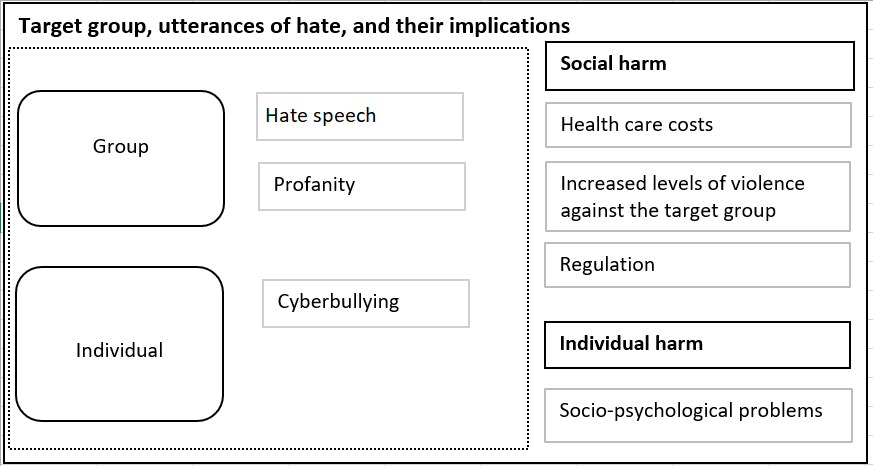
\includegraphics{degrees_harm.PNG}\\

\begin{tabular}{ |p{7cm}||p{3cm}|p{3cm}|p{1cm}| }
 \hline
 \multicolumn{4}{|c|}{Overview definitions of hate speech 2017 - 2020} \\
 \hline
 Definition of hate &Target & Author & Year \\
 \hline
 Language that is used to expresses hatred towards a targeted group or is intended to be derogatory, to humiliate,
or to insult the members of the group & Group    &\citet{Davidson2017AutomatedLanguage} & 2017  \\
           &     &   & \\
 Any emotional expression imparting opinions or
ideas – bringing a subjective opinion or idea to an
external audience- with discriminatory purposes. It
can take many forms: written, non-verbal, visual,
artistic, and may be disseminated through any media,
including internet, print, radio, or television &An external audience (group) & \citet{Martins2018HateAnalysis} & 2018\\
     & & &\\
Any communication that disparages a person or a group
on the basis of some characteristic such as race,
color, ethnicity, gender, sexual orientation, nationality, religion, or other characteristics&   Individual OR group  & \citet{Nockleby2000HATESPEECH}; \citet{Bauwelinck2019LT3hatEval} &2000; 2019\\
    & & & \\
 Online hate is composed of the use of language that contains either hate speech targeted toward individuals or groups, profanity, offensive language, or toxicity –
in other words, comments that are rude, disrespectful, and can result in negative online and offline consequences for the individual, community, and society at large & Individual OR group  & \citet{Salminen2020DevelopingPlatforms} &2020\\
 \hline
\end{tabular}\\
\break{} 
\textbf{3.3 Methods for detecting online hate speech}\\
\break{}
\textbf{3.3.1 Lexical methods for identifying hate}\\
\break{}
The use of online hate speech is wide-spread across multiple platforms, but for the scope of this thesis this study will solely focus on Twitter. One way to detect hate speech in tweets is by using key-words for detecting online hateful language. For this purpose, the hate speech lexicon Hatebase was developed. This is a database that consists of hateful words that can be used to filter hate speech words from social media platforms, with the goal to predict regional violence as a consequence of hate speech \footnote{https://hatebase.org/}. \\

\citet{Davidson2017AutomatedLanguage} used the Hatebase lexicon as keywords to crawl Twitter data. They obtained 25k tweets that contained hateful words from this repository, which they then for accuracy purposes have had annotated by human workers of Appen  \cite{Davidson2017AutomatedLanguage}. Out of all filtered hate words, only 5\% of the tweets were manually coded as hate speech, which shows the imprecision of Hatebase and the problem with lexical methods. \\
\break{}\
\textbf{3.3.2 Classification algorithms based on multiple labels}\\
\break{}
In the field of hate speech detection on Twitter data, several relevant studies have been done.  In 2017, \citet{SchmidtAProcessing} did a study on existing methods for hate speech detection. They explained that lexical methods are often used as a baseline for developing methods on restricting online hate. 

They found that character-level approaches work better than token-level approaches and that lexicon resources might work well in combination with other methods. 

Malmasi \& Zampieri (2017) did a research on methods to detect hate speech on social media. Thereby they made a distinction between hate speech and profanity. The dataset they used consisted of tweets they annotated with the categories 'HATE', 'OFFENSIVE' and 'OK'. They also applied standard lexical features and a linear SVM classifier as a starting point for their study. Their results show that a character 4-gram model gave the best results, but that discriminating hate speech from profanity remains a difficult task. In 2018 they conducted the same research but with a different dataset. Malmasi \& Zampieri make use of N-grams, skip grams and clustering-based word representations. They conclude again that discriminating hate speech from profanity is very hard and that the standard features they applied might not be enough for telling them apart with high certainty.

Gomez' research (2018) is partly build on the findings of Malmasi \& Zampieri. They use NLP techniques and emotion analysis for hate speech classification. In their study they apply a combination of lexicon-based and machine learning approaches to forecast hate speech in a text by means of a sentiment analysis that focused on detecting feelings. They conclude that the inclusion of emotions into the model improved the certainty on hate speech detection.\todo{rewrite this entire sub paragraph about classification}\\

% Sentiment Analysis emotion classification methods\\

% With regards to sentiment analysis and political tweets, relevant work has been done by Bhattacharya et al. (2010), Murthy et al. (2015) and Liu \& Lei Lei (2018). 

% Bhattacharya et al. focus on the public opinion of the 2012 US elections on Twitter. They assess statements of opinions related to the personality traits of politicians. They used Amazon Mechanical Turk for the annotation of \emph{positive}, \emph{negative} and \emph{neutral} personality traits of presidential candidates. Twitter data was collected with Twitter Search API by using keywords. Even though the topic differs from the subject of analysis in this thesis, there are similarities in the domain that is being examined. Therefore, the methods that are used can be relevant for the analysis of the Tweets in this thesis.

% Liu \& Lei Lei focus on the speeches of Trump and Clinton by means of sentiment analysis. They compare speech themes of Clinton and Trump with the rhetoric strategies used in their speeches. The data was collected through the UC Santa Barbara's (2017) "The Presidency Project" website. They execute "a sentence-level lexicon-based sentiment analysis". Thereby they make use of a program in R called \emph{syuzhet} (Jockers, 2017). They furthermore use two different lexicons, Jockers'(2017b) and Liu at al.'s (2005) sentiment lexicon to make the outcome of their findings more trustworthy. These methods are relevant, because they can be applied to the topic of this thesis as well.\\

\section{Methodology}
%Methodology **(20)**
%	5. Do I get a clear picture of the used resources?
%		5. E.g., for data, do I get a clear picture of the data, its state, its availability, how much it is, how dirty, how much work to process, etc, etc.
%	6. Are the methods which will be used described in enough detail, so that I can picture what will be done exactly? 
%	7. Is the evaluation appropriate? That is, do I understand how each subquestion is answered by the evaluation? 

\textbf{4.1 Dataset}\\
\break
For the purpose of this research the tool Trump Twitter Archive\footnote{http://www.trumptwitterarchive.com/} will be used. This is a large database that contains every tweet of the Twitter account @realDonaldTrump ranging from 2009 until today. It enables a user to search for tweets during a specific time period based on keywords. The Trump campaign started on June the 16th 2015. This is the starting point of the dataset. The dataset was searched on the 12th of May 2020. This is the end date that will be used to analyze tweets from the @realDonaldTrump account. Retweets and hashtags will be removed from the dataset. In this way only the tweet ID, the text and the date are left. + amount of tweets every year + average number of tweets + average number of words\\
\break{}

\begin{center}
\begin{tabular}{ c c}
 The amount of tweets for every year &   \\ 
 2015 & x \\  
 2016 & x \\
 2017 & x    \\
 2018 & x    \\
 2019 & x    \\
 2020 & x    \\
\end{tabular}
\end{center} \\

\textbf{4.2 Pre-processing}\\
\break{}
\textbf{4.2.1 Keyword-based filtering}\\
\break{}
Existing hate speech lexicons such as Hasebase.org will not be used for this research, due to inconsistencies and contradictions in the labelling process (Davidson, 2017). Therefore, in this research the tweets will be filtered based on keywords that could potentially be associated with higher levels of hate speech. For the purpose of this research and the limited time scope, only tweets that could be hateful towards groups of people will be analyzed. Any hateful language that is aimed at a single individual will not be taken in consideration in this case. The groups of people mentioned in Trump's tweets that often are associated with higher levels of hate are: immigrants, certain religions and specific countries or nationalities (source; source). Therefore, the keywords that are used to filter this dataset are: \\
\break{}
Mexico - Mexican - Mexicans - immigrant - immigrants - Hispanic - Hispanics - Muslim - Muslims - Islam - rapist - rapists - ISIS - gang member - gang members - blacks - why don’t they do back - bring them back from where they came - these aren’t people - human traffickers - coyotes - invasion -  infestation - abuser - shithole countries - terrorist - terrorists - rats -  migrant - migrants - refugee - refugees - congresswomen - cartel - cartels -  China - Chinese virus - viciously telling the people of the United States -  you can’t leave fast enough \\
\break{}
After filtering the tweets based on these keywords a dataset containing 1300 tweets is left. This set of tweets will be used for data-labelling.\\
\break{}
\textbf{4.2.2 Gold Standard: Human annotation based on multiple labels with Swivl}\\
\break{}
The next step of pre-processing is annotation of the data. Annotation of the data will be done manually by three people with respectively a background in Literature Studies, Communication \& Media Studies and Cultural Studies. These people are selected, because their backgrounds are relevant with regards to either language or the topics mentioned in the tweets. \\
\break{}
In line with the research of Davidson (2017) the data will be labelled according to three classes: HATE SPEECH, OFFENSIVE LANGUAGE and NEUTRAL. The annotators will be given the task to look at each tweet separately and rate them based on a scale from 0 to 2, where HATE gets the label 0 and NEUTRAL the label 2. In order to make the annotation process a slightly less hazardous task, the data annotation tool Swivl will be used. This tool provides an interface for the annotators to label the data according to existing hate speech guidelines adapted to fit the purpose of this research project.\\
\break{}
\textbf{4.3 Baseline models}\\
Keyword-based classifier (KBC) AND the static model \footnote{https://bitbucket.org/ceshwar/bag-of-communities/src/master/}
OR Logistic regression and linear SVM\\
\break{}
\textbf{4.2 Simple feature extraction}

\begin{center}
 \begin{tabular}{||c c||} 
 \hline
 Feature & Definition \\ [0.5ex] 
 \hline\hline
 Number\_of\_tweets & Average number of tweets in the document \\ 
 \hline
 Number\_of\_words\_per\_tweet & Average number of words per tweet\\
 \hline
 Number\_of\_words\_all\_tweets & Average number of words all tweets\\
 \hline
 Uppercase\_per\_tweet & Average number of uppercase characters per tweet\\
 \hline
Exclamation\_marks\_per\_tweet & Average number of exclamation marks per tweet\\ [1ex] 
 \hline
\end{tabular}
\end{center}

\textbf{4.4 Pre-training the classifier}\\
\break{}
\textbf{4.5 BERT}\\
\break{}
\section{Results}
%Risk assessment **(10)**
%	* Is it complete? Is is realistic? Is the backup plan executable?
\section{Discussion \& conclusion}\\
xxx
\maketitle



\medskip

\bibliography{references}
\end{document}



